\documentclass[10pt, compress]{beamer}

\usetheme{m}

\usepackage{booktabs}
\usepackage[scale=2]{ccicons}
\usepackage[outputdir=.texpadtmp]{minted}
\usepackage{FiraSans}
\usepackage{graphicx}
\usepackage{caption}
\usepackage{subcaption}
\usepackage{todonotes}
\usepackage{listings}
\usepackage{tikz}

\usemintedstyle{trac}

\title{Lichtsteuerungsautomatisierung}
\subtitle{Projekt: DV-Anwendungen in der Technik}
\date{\today}
\author{Schuller, Thiemann, Wildt\\
  Betreuer: Prof. Dr. Franz Josef Schmitt}
\institute{Hochschule Rosenheim}

\begin{document}

\maketitle

\section{Grundlagen}

\plain{ }{
  \vspace{-2em}
  \begin{center}
    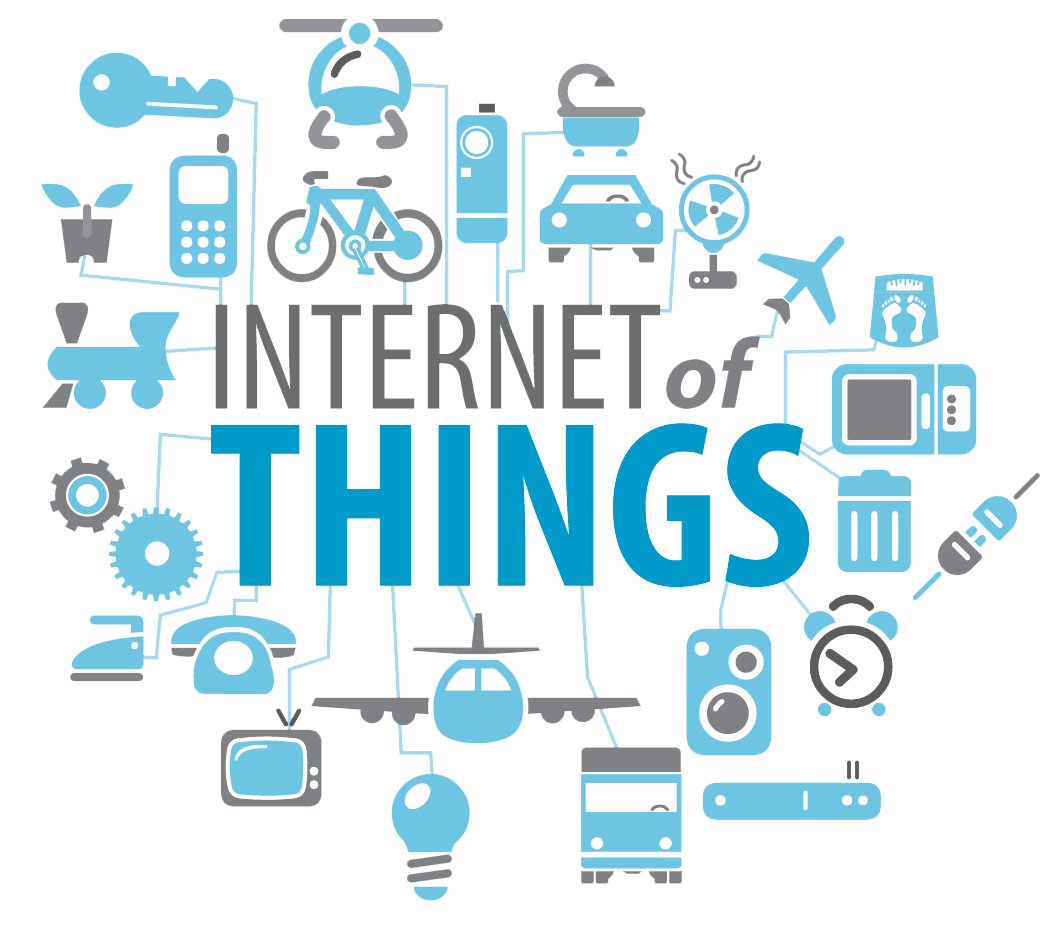
\includegraphics[width=0.9\textwidth]{images/iot}
  \end{center}
}

\plain{ }{
  \vspace{-2em}
  \begin{center}
    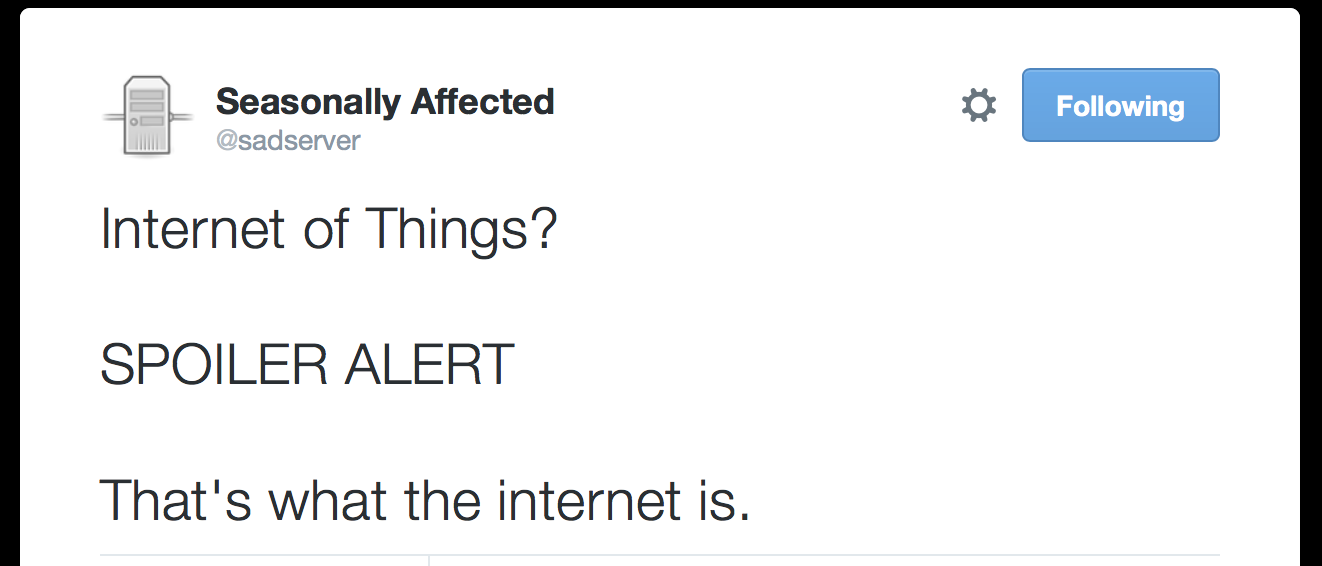
\includegraphics[width=0.75\textwidth]{images/sadserver1}
  \end{center}
}


\section{Hardware}

\begin{frame}{Hardware - Raspberry Pi 2}
  \begin{center}
    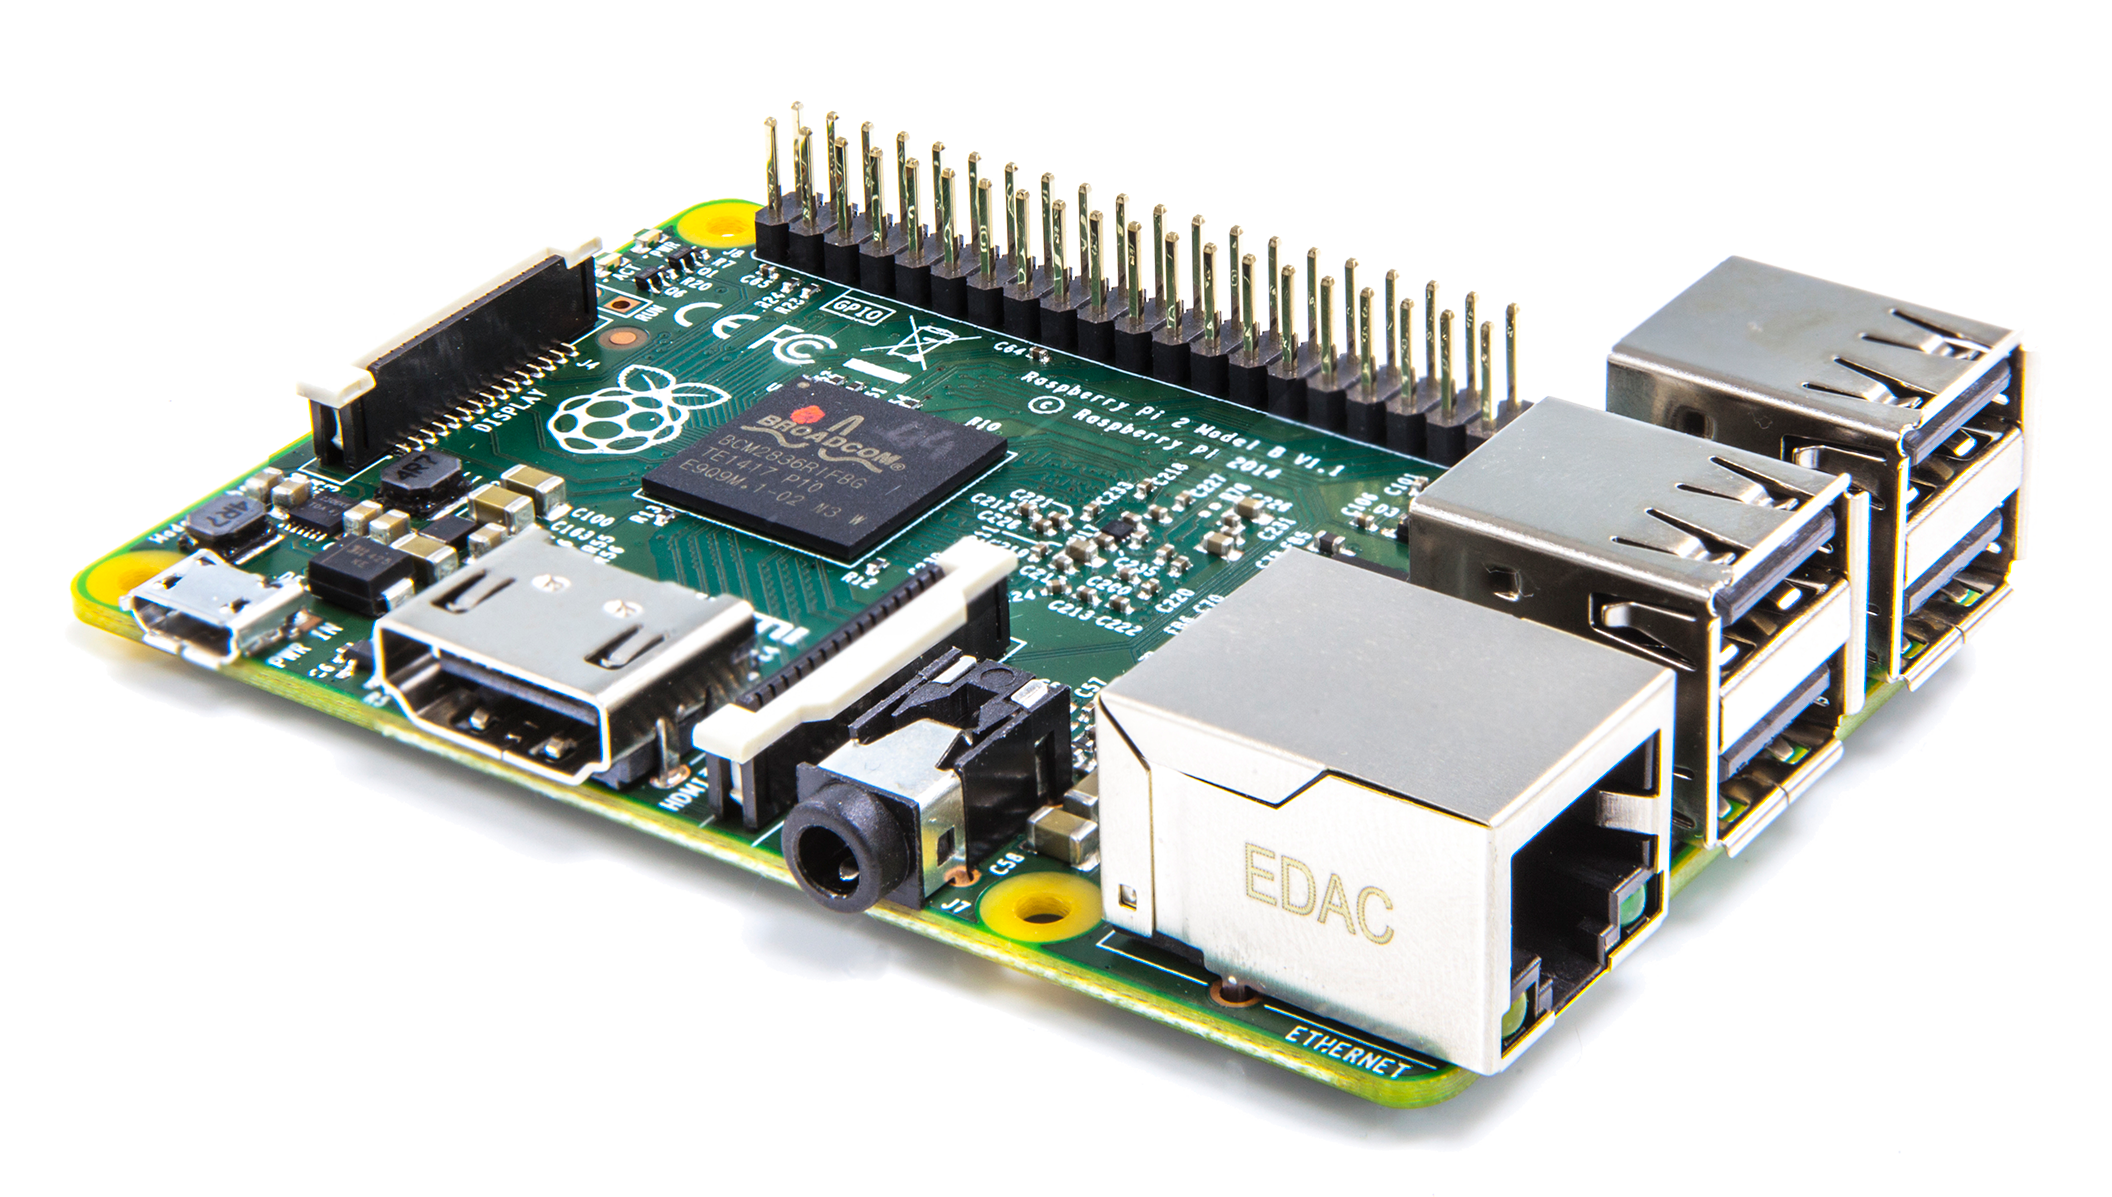
\includegraphics[width=\textwidth]{images/rpi2}
    \label{fig:rpi}
  \end{center}
\end{frame}

\begin{frame}{Hardware - Raspberry Pi 2 - Gründe}
  \Large
  \begin{itemize}
    \item Universell einsetzbar
    \item Sehr gutes Preis/Leistungs-Verhältnis
    \item Umfangreicher Support durch Community
    \item Große Basis unterstützter Software
    \item Einfach in der Handhabung
  \end{itemize}
\end{frame}

\begin{frame}{Hardware - Raspberry Pi 2 - Specs}
  \Large
  \center{
  \begin{tabular}{ l r }
%    L/B/H & \texttt{9,3 x 6,4 x 2,0 cm}\\
%    Gewicht & \texttt{45 g}\\
%    \\
    CPU & \texttt{ARM Cortex-A7}\\
    CPU-Kerne & \texttt{4}\\
    CPU-Takt & \texttt{900 MHz}\\
    RAM & \texttt{1 GB}\\
    \\
    Stromverbrauch & \texttt{max. 4 W} \\
    Preis & \texttt{\textasciitilde 40€}
  \end{tabular}}

\end{frame}

\begin{frame}{Hardware - RaspBee}
  \begin{center}
    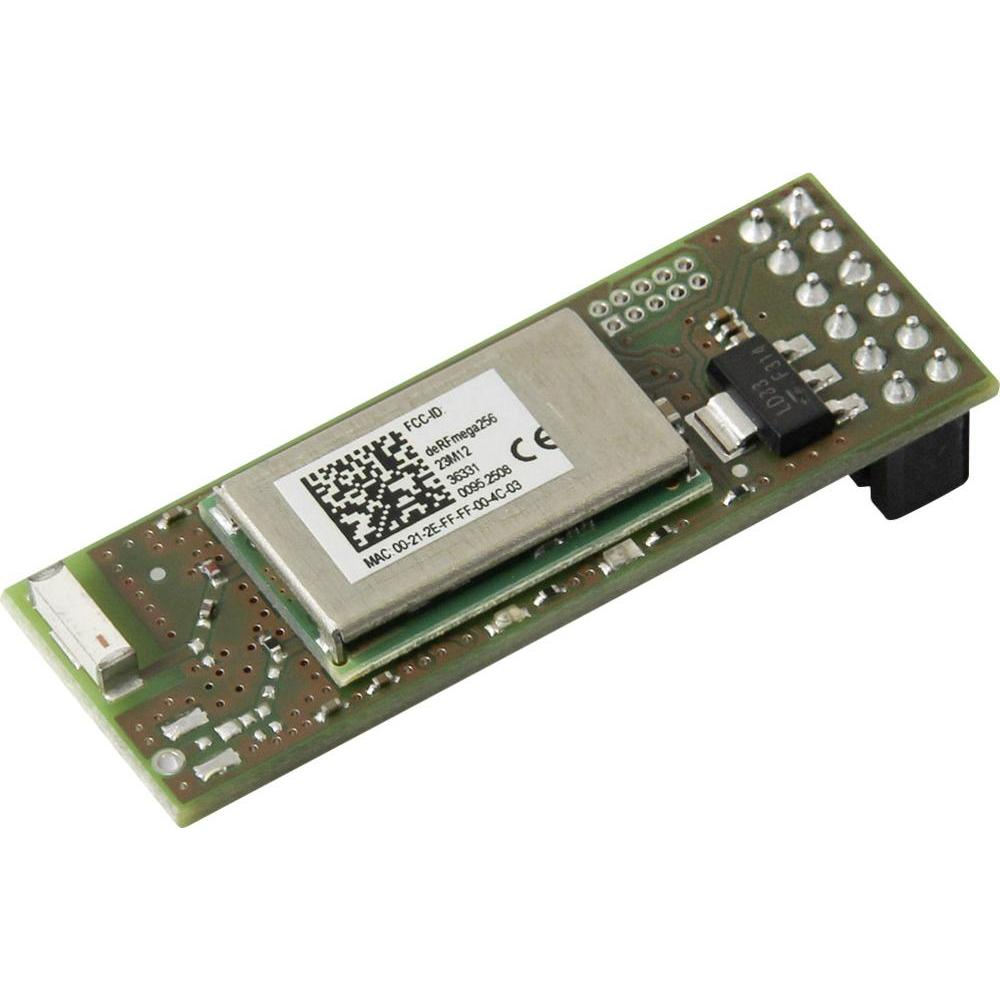
\includegraphics[width=\textwidth]{images/raspbee}
    \label{fig:rbee}
  \end{center}
\end{frame}

\begin{frame}{Hardware - RaspBee - Gründe}
  \Large
  \begin{itemize}
    \item Sehr gute Unterstützung für RPIs
    \item Komplette Verwaltungssoftware
    \item Gute Verfügbarkeit
    \item Weit verbreitet
  \end{itemize}
\end{frame}

\begin{frame}{Hardware - Hue}
  \begin{center}
    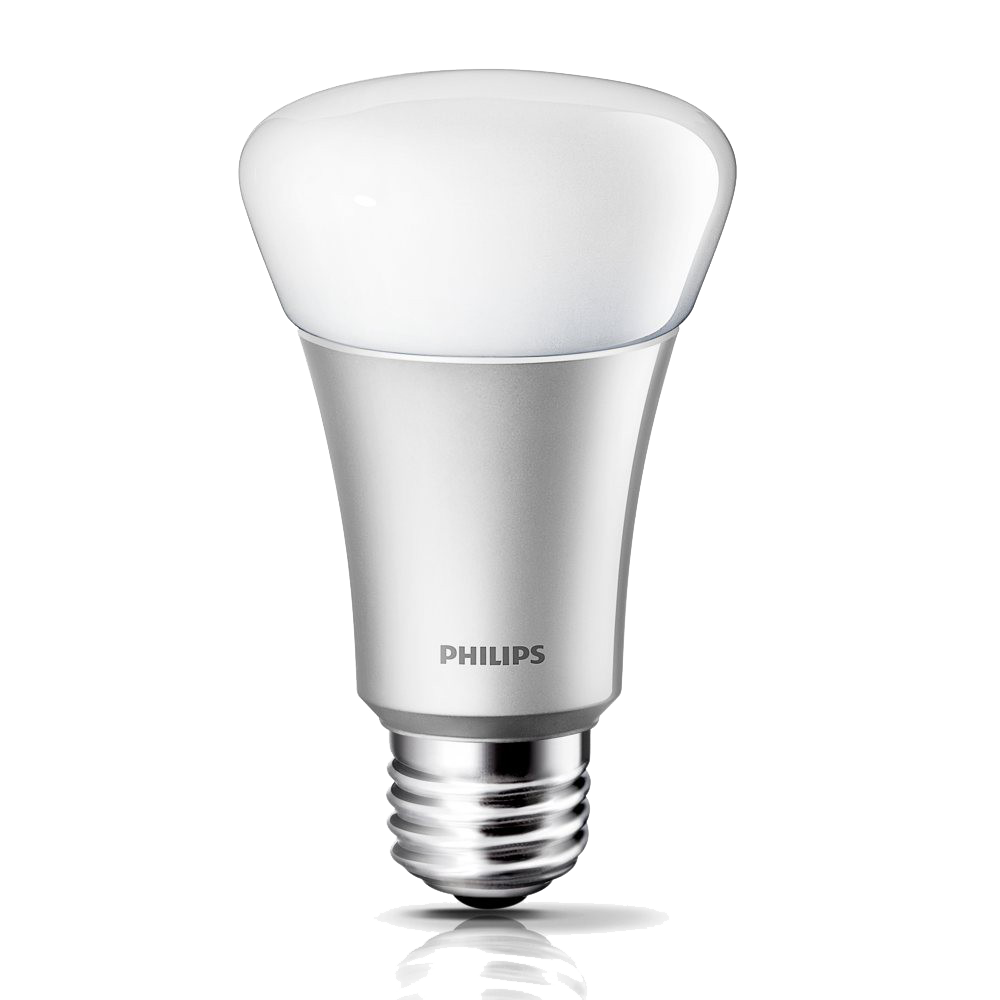
\includegraphics[width=0.7\textwidth]{images/hue}
    \label{fig:hue}
  \end{center}
\end{frame}

\begin{frame}{Hardware - Hue - Gründe}
  \Large
  \begin{itemize}
    \item Weite Verbreitung
    \item Gute Erfahrungen
    \item Gute Qualität
  \end{itemize}
\end{frame}

\section{Software}

\begin{frame}{Software - RaspBee}
  \Large
  \begin{itemize}
    \item GCFFlasher
    \begin{itemize}
      \Large
      \item Firmware-Tool für RaspBee
      \item Flashen und Reset des Moduls
      \item Von uns nicht verwendet
      \newline
    \end{itemize}
	\item deCONZ\\
      \normalsize{\textit{\textbf dresden \textbf electronic \textbf{Con}trol
        \textbf Zigbee Appliances}}
    \begin{itemize}
      \Large
      \item Desktop Applikation
      \item Web Applikation
      \item REST API
    \end{itemize}
  \end{itemize}
\end{frame}

\begin{frame}{Software - deCONZ - Desktop Applikation}
  \Large
  Hardwarenahe Steuerung von ZigBee-Nodes
  \begin{center}
    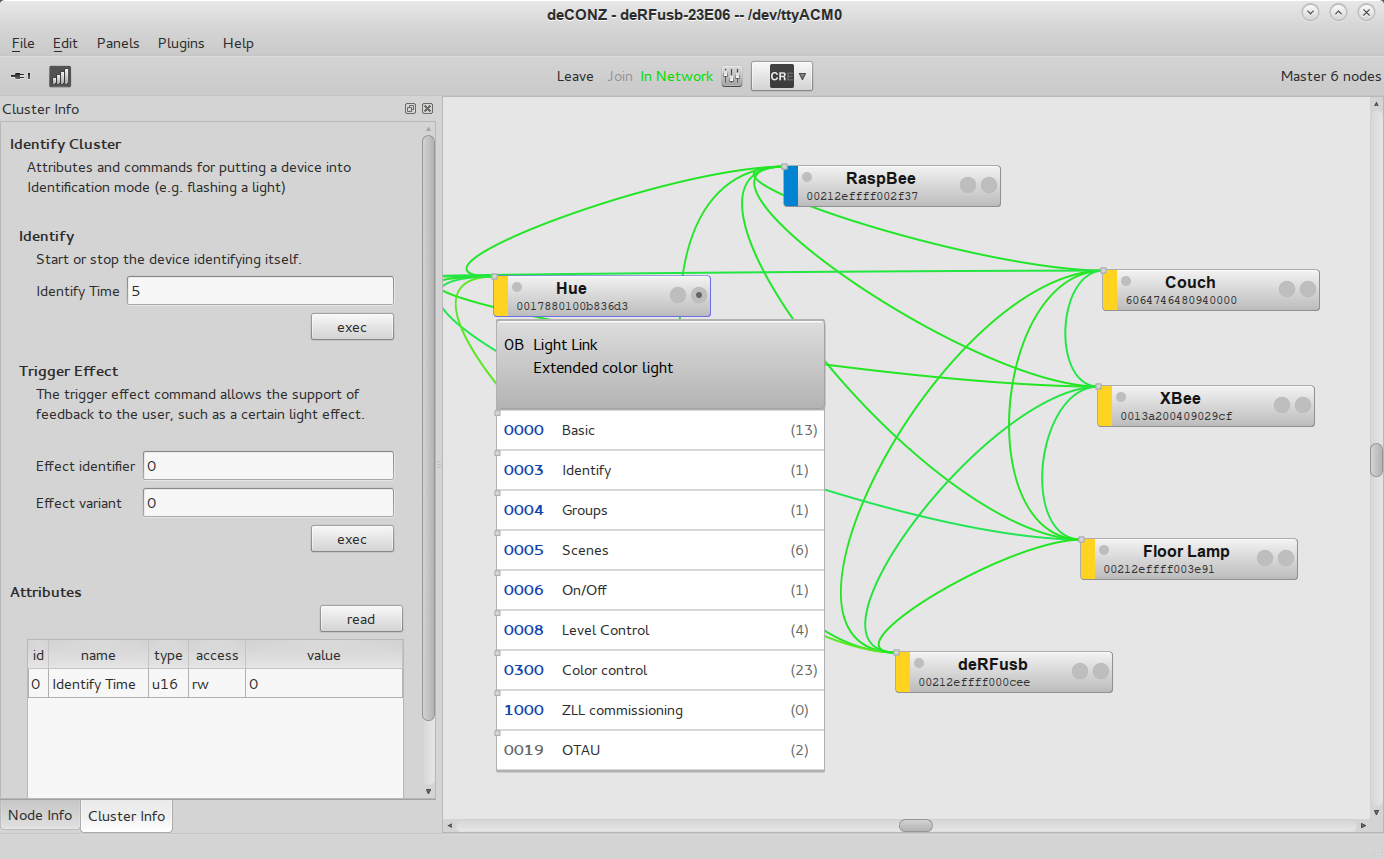
\includegraphics[width=0.8\textwidth]{images/deconz_app}
  \end{center}
\end{frame}

\begin{frame}{Software - deCONZ - Web Applikation}
  \Large
  Steuerung der Beleuchtung über den Browser
  \begin{center}
    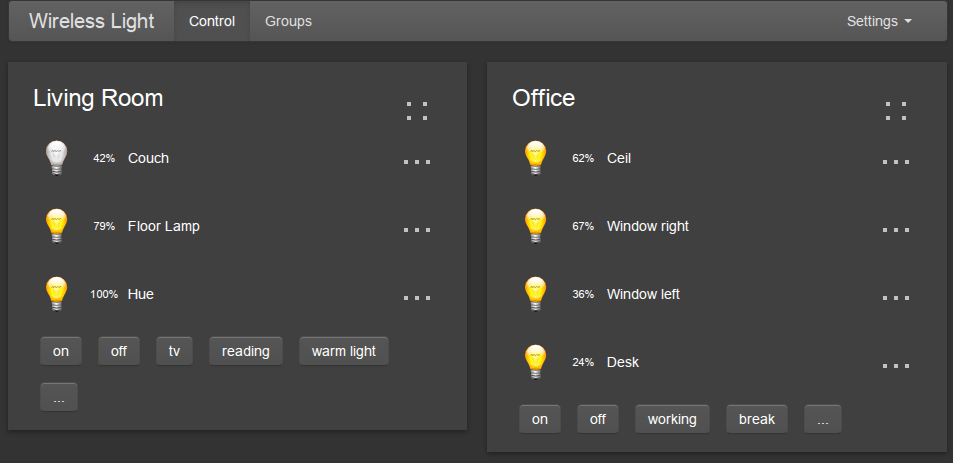
\includegraphics[width=0.8\textwidth]{images/deconz_web}
  \end{center}
  unter Nutzung der REST-API
\end{frame}



\section{Was wir machen wollten}

\begin{frame}{Projekt - Idee}
  \begin{center}
    
\includegraphics[width=0.9\textwidth]{images/grobarchitektur}
  \end{center}
\end{frame}

\section{Was wir dann gemacht haben}

\begin{frame}{Projekt - Realität}
  \begin{center}
    
\includegraphics[width=0.9\textwidth]{images/realworld}
  \end{center}
\end{frame}

\section{Demo time!}

\input{demo.tex}

\section{Sicherheitsaspekte}

\begin{frame}{Sicherheitslücken in der Logik}
  \begin{quote}
    \normalsize
    By causing a failure condition in the 2.4 GHz radio frequency band,
    the security system \textbf{does not fail closed} with an assumption that an
    attack is underway. Instead, \textbf{the system fails open}, and the security
    system continues to report that "\alert{All sensors are in-tact and all doors
    are closed. No motion is detected.}"
    \begin{flushright}
      \small
      -- Rapid7 (05.01.2016), \href{https://community.rapid7.com/community/infosec/blog/2016/01/05/r7-2015-23-comcast-xfinity-home-security-system-insecure-fail-open}{R7-2015-23}
    \end{flushright}
  \end{quote}
\end{frame}

\begin{frame}{Sicherheitslücken im Protokoll}
  \begin{quote}
    \normalsize
    \textbf{Verschlüsselung als Satire}\\
    Grundsätzlich kommunizieren die Geräte verschlüsselt.
    Jedoch schreibt das ZigBee-Konsortium vor, dass alle Geräte
    \alert{ein und dasselbe Schlüsselpaar} (Fallback Key) kennen
    und akzeptieren müssen – und dieses asymmetrische Schlüsselpaar ist
    \alert{öffentlich bekannt}.
    \begin{flushright}
      \small
      -- \url{http://heise.de/-3010287}
    \end{flushright}
  \end{quote}
\end{frame}

\begin{frame}{}
  \begin{center}
    \makebox[\textwidth][c]{
\includegraphics[width=1\paperwidth]{images/zigbee}}

    \url{http://www.zigbee.org}
  \end{center}
\end{frame}

\begin{frame}{}
  \begin{center}
    \vspace{-0.2cm}
    \makebox[\textwidth][c]{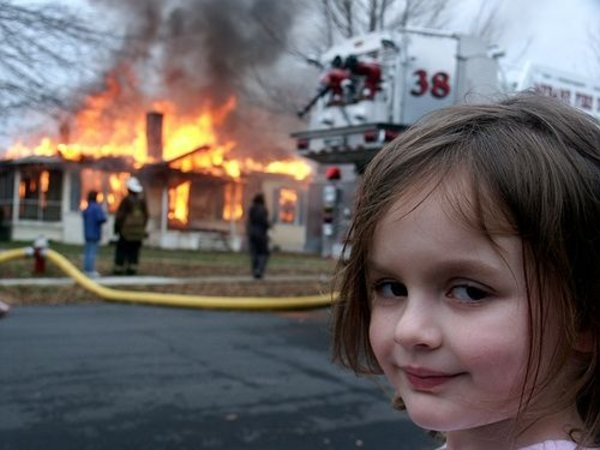
\includegraphics[width=1\paperwidth]{images/desastergirl}}
    \label{fig:disaster}
  \end{center}
\end{frame}


\begin{frame}{Final}

  \begin{center}\huge Fragen?\end{center}
    
  \vspace{1cm}
  \begin{center}
  {\small

  The \LaTeX \ theme \emph{mtheme} is licensed under a
  \href{http://creativecommons.org/licenses/by-sa/4.0/}{Creative Commons
  Attribution-ShareAlike 4.0 International License}.}

  \ccbysa
  
  \end{center}

\end{frame}

\begin{frame}{Grafiken}
  \begin{itemize}
    \item \small{Internet of Things (Folie \pageref{fig:iot}):}\\
      \footnotesize{
        \url{http://brilliency.com/tag/internet-of-things/}
      }
    \item \small{SPOILER ALERT (Folie \pageref{fig:spoiler}):}\\
      \footnotesize{
        \url{https://twitter.com/sadserver/status/621382996323536896}
      }
    \item \small{RPI2 (Folie \pageref{fig:rpi}):}\\
      \footnotesize{
        \url{https://www.raspberrypi.org/blog/raspberry-pi-2-on-sale/}
      }
    \item \small{RaspBee (Folie \pageref{fig:rbee}):}\\
      \footnotesize{
        \url{https://www.conrad.de/de/raspbee-1369408.html}
      }
    \item \small{Philips Hue LED Leuchte (Folie \pageref{fig:hue}):}\\
      \footnotesize{
        \url{http://www.homewizard.co.uk/philips-hue-led-lamp-single-pack.html}
      }
  \end{itemize}
  
\end{frame}

\end{document}